\documentclass[11pt,a4paper]{article}
\usepackage[margin=2cm]{geometry}
\usepackage[T1]{fontenc}
\usepackage[utf8]{inputenc}
\usepackage{hyperref}
\usepackage{xcolor}
\usepackage{listings}
\usepackage{tikz}
\usetikzlibrary{positioning,arrows.meta}
\definecolor{codebg}{RGB}{248,250,252}
\definecolor{codeblue}{RGB}{37,99,235}
\definecolor{codegreen}{RGB}{22,101,52}
\definecolor{codered}{RGB}{185,28,28}
\definecolor{codegray}{RGB}{100,116,139}
\lstdefinelanguage{JavaScript}{morekeywords={const,let,var,async,await,function,try,catch,return,if,else,for,of,require,module,exports},sensitive=true,morecomment=[l]{//},morestring=[b]",morestring=[b]`}
\lstdefinestyle{prokuraCode}{basicstyle=\ttfamily\small,breaklines=true,frame=single,columns=fullflexible,keepspaces=true,showspaces=false,showstringspaces=false,showtabs=false,tabsize=2,numbers=left,numberstyle=\tiny\color{codegray},keywordstyle=\color{codeblue}\bfseries,stringstyle=\color{codered},commentstyle=\color{codegreen},rulecolor=\color{codegray},backgroundcolor=\color{codebg}}
\lstset{style=prokuraCode}
\newcommand{\docheader}[2]{
\begin{titlepage}
\centering
{\Large\bfseries Prokura HoReCa Supply\par}
\vspace{0.4cm}
{\large Dokumentasi Fitur Microservice Final Project\par}
\vspace{0.8cm}
{\large Mata Kuliah: Proyek 2 - Final Project\par}
\vspace{1.2cm}
{\large\bfseries #1\par}
{\large NIM: #2\par}
\vfill
\begin{tabular}{rl}
Program Studi: & Ilmu Komputer\\
Departemen: & Departemen Ilmu Komputer dan Elektronika (DIKE)\\
Fakultas: & FMIPA\\
Universitas: & Universitas Gadjah Mada\\
\end{tabular}
\vfill
\end{titlepage}
}

\begin{document}
\docheader{Pison Golda Mountera}{24/543770/PA/23107}

\section*{Peran}
Owner Reporting Service. Pison bertanggung jawab pada rekap penjualan, KPI transaksi, top produk, top customer, dan ringkasan admin.

\section*{Bukti Microservice}
Reporting Service berada di \path{prokura-api/src/services/reporting} dan dapat dijalankan sebagai service tersendiri melalui \texttt{service-host}.

\begin{lstlisting}[language=JavaScript]
const serviceRegistry = {
  catalog: registerCatalogRoutes,
  customer: registerCustomerRoutes,
  inventory: registerInventoryRoutes,
  order: registerOrderRoutes,
  reporting: registerReportingRoutes,
};
\end{lstlisting}

Penjelasan: entry \texttt{reporting: registerReportingRoutes} membuktikan Reporting Service punya boundary sendiri. Pada Docker Compose microservices, service ini berjalan di port \texttt{5105}.

\section*{Tanggung Jawab Fitur}
\begin{enumerate}
\item Rekapitulasi penjualan.
\item Analitik top produk dan top customer.
\end{enumerate}

\section*{Diagram Tabel yang Ditangani}
\begin{center}
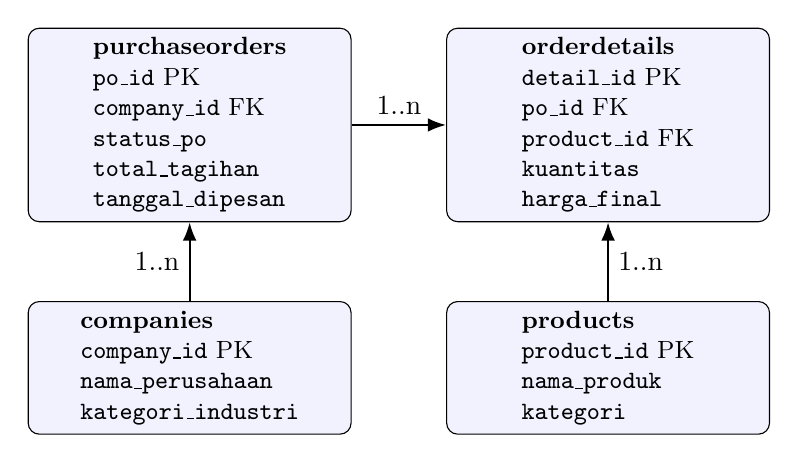
\begin{tikzpicture}[entity/.style={draw, rounded corners, fill=blue!5, align=left, font=\small, minimum width=4.1cm}, rel/.style={-Latex, thick}]
\node[entity] (po) {\textbf{purchaseorders}\\\texttt{po\_id} PK\\\texttt{company\_id} FK\\\texttt{status\_po}\\\texttt{total\_tagihan}\\\texttt{tanggal\_dipesan}};
\node[entity, right=1.2cm of po] (details) {\textbf{orderdetails}\\\texttt{detail\_id} PK\\\texttt{po\_id} FK\\\texttt{product\_id} FK\\\texttt{kuantitas}\\\texttt{harga\_final}};
\node[entity, below=1.0cm of details] (products) {\textbf{products}\\\texttt{product\_id} PK\\\texttt{nama\_produk}\\\texttt{kategori}};
\node[entity, below=1.0cm of po] (companies) {\textbf{companies}\\\texttt{company\_id} PK\\\texttt{nama\_perusahaan}\\\texttt{kategori\_industri}};
\draw[rel] (companies) -- node[left]{1..n} (po);
\draw[rel] (po) -- node[above]{1..n} (details);
\draw[rel] (products) -- node[right]{1..n} (details);
\end{tikzpicture}
\end{center}

Penjelasan: Reporting Service membaca \texttt{purchaseorders}, \texttt{orderdetails}, \texttt{products}, dan \texttt{companies}. Service ini tidak mengubah data, tetapi menggabungkan tabel transaksi dan master data untuk menghasilkan KPI, top produk, dan top customer.

\section*{Lokasi Kode Program dan Penjelasan}
\subsection*{Route laporan}
Lokasi kode: \path{prokura-api/src/services/reporting/routes.js}. \texttt{GET /api/admin/summary}: line 5. \texttt{GET /api/reports/sales}: line 14.

\begin{lstlisting}[language=JavaScript]
app.get("/api/admin/summary", async (_req, res) => {
  try {
    const summary = await getAdminSummary(pool);
    res.json({ success: true, data: summary });
  } catch (error) {
    sendError(res, error, "Gagal mengambil ringkasan admin");
  }
});
\end{lstlisting}

Penjelasan: endpoint ini memberi ringkasan cepat untuk dashboard admin, seperti jumlah perusahaan, produk, order, dan order pending.

\begin{lstlisting}[language=JavaScript]
app.get("/api/reports/sales", async (req, res) => {
  try {
    const { start, end } = normalizeDateRange(req.query);
    const report = await getSalesReport(pool, { start, end });

    res.json({
      success: true,
      data: report,
    });
  } catch (error) {
    sendError(res, error, "Gagal mengambil laporan penjualan");
  }
});
\end{lstlisting}

Penjelasan: endpoint laporan menerima rentang tanggal, menormalisasi tanggal, lalu mengambil data sales report dari repository. Response berisi summary, tren bulanan, segment revenue, top products, top clients, dan transaksi.

\subsection*{SQL repository reporting}
Lokasi kode: \path{prokura-api/src/services/reporting/repository.js}. Summary sales: line 17. Top products: line 56. Top clients: line 73. Transactions report: line 91.

\begin{lstlisting}[language=JavaScript]
const summary = await pool.query(
  `
    SELECT COUNT(*)::int AS total_po,
           COALESCE(SUM(total_tagihan), 0)::float AS total_revenue,
           COALESCE(AVG(total_tagihan), 0)::float AS avg_po,
           COUNT(DISTINCT company_id)::int AS klien_aktif
    FROM purchaseorders
    WHERE DATE(tanggal_dipesan) BETWEEN $1 AND $2
      AND status_po != 'Cancelled'
  `,
  params,
);
\end{lstlisting}

Penjelasan: query ini menghitung KPI utama laporan: total PO, total revenue, rata-rata nilai PO, dan jumlah klien aktif. Order dengan status \texttt{Cancelled} tidak dihitung sebagai penjualan.

\begin{lstlisting}[language=JavaScript]
const monthly = await pool.query(
  `
    SELECT TO_CHAR(tanggal_dipesan, 'YYYY-MM') AS bulan,
           SUM(total_tagihan)::float AS revenue,
           COUNT(*)::int AS jumlah_po
    FROM purchaseorders
    WHERE DATE(tanggal_dipesan) BETWEEN $1 AND $2
      AND status_po != 'Cancelled'
    GROUP BY TO_CHAR(tanggal_dipesan, 'YYYY-MM')
    ORDER BY bulan ASC
  `,
  params,
);
\end{lstlisting}

Penjelasan: query ini mengelompokkan revenue dan jumlah PO per bulan. Data ini dipakai untuk grafik tren penjualan.

\begin{lstlisting}[language=JavaScript]
const topProducts = await pool.query(
  `
    SELECT p.nama_produk AS produk, p.kategori,
           SUM(od.kuantitas)::int AS total_qty,
           SUM(od.kuantitas * od.harga_final)::float AS revenue
    FROM orderdetails od
    JOIN products p ON od.product_id = p.product_id
    JOIN purchaseorders po ON od.po_id = po.po_id
    WHERE DATE(po.tanggal_dipesan) BETWEEN $1 AND $2
      AND po.status_po != 'Cancelled'
    GROUP BY p.product_id
    ORDER BY total_qty DESC
    LIMIT 10
  `,
  params,
);
\end{lstlisting}

Penjelasan: query ini mencari produk terlaris berdasarkan total kuantitas. Join ke \texttt{products} memberi nama produk dan kategori, sedangkan join ke \texttt{purchaseorders} memastikan filter tanggal dan status diterapkan.

\begin{lstlisting}[language=JavaScript]
const topClients = await pool.query(
  `
    SELECT c.nama_perusahaan AS klien, c.kategori_industri AS segmen,
           COUNT(po.po_id)::int AS jumlah_po,
           SUM(po.total_tagihan)::float AS revenue
    FROM purchaseorders po
    JOIN companies c ON po.company_id = c.company_id
    WHERE DATE(po.tanggal_dipesan) BETWEEN $1 AND $2
      AND po.status_po != 'Cancelled'
    GROUP BY c.company_id
    ORDER BY revenue DESC
    LIMIT 10
  `,
  params,
);
\end{lstlisting}

Penjelasan: query ini mencari customer dengan revenue tertinggi. Hasilnya dipakai untuk grafik atau tabel top customer.

\subsection*{UI admin laporan}
Lokasi kode: \path{prokura-admin/app3.py}. Menu \texttt{Laporan \& Analitik}: line 912. Fetch report \texttt{/api/reports/sales}: line 924.

Penjelasan: UI admin memilih rentang tanggal dan memanggil endpoint Reporting Service. UI tidak menghitung langsung dari database.

\section*{SQL Query Demo dan Penjelasan}
\subsection*{Query 1: rekapitulasi penjualan}
\begin{lstlisting}[language=SQL]
SELECT COUNT(*) AS total_po,
       COALESCE(SUM(total_tagihan), 0) AS total_revenue,
       COALESCE(AVG(total_tagihan), 0) AS avg_po,
       COUNT(DISTINCT company_id) AS klien_aktif
FROM purchaseorders
WHERE DATE(tanggal_dipesan) BETWEEN '2026-01-01' AND '2026-12-31'
  AND status_po != 'Cancelled';
\end{lstlisting}
Penjelasan: query ini menghitung KPI sales dalam rentang tahun 2026. \texttt{COALESCE} membuat nilai agregat menjadi 0 jika belum ada order pada rentang tersebut.

\subsection*{Query 2: analitik top produk}
\begin{lstlisting}[language=SQL]
SELECT p.nama_produk AS produk, p.kategori,
       SUM(od.kuantitas) AS total_qty,
       SUM(od.kuantitas * od.harga_final) AS revenue
FROM orderdetails od
JOIN products p ON od.product_id = p.product_id
JOIN purchaseorders po ON od.po_id = po.po_id
WHERE DATE(po.tanggal_dipesan) BETWEEN '2026-01-01' AND '2026-12-31'
  AND po.status_po != 'Cancelled'
GROUP BY p.product_id
ORDER BY total_qty DESC
LIMIT 10;
\end{lstlisting}
Penjelasan: query ini menghitung produk terlaris dari detail order. \texttt{SUM(od.kuantitas)} menentukan ranking, sedangkan \texttt{SUM(od.kuantitas * od.harga\_final)} menghitung revenue produk.

\subsection*{Query 3: analitik top customer}
\begin{lstlisting}[language=SQL]
SELECT c.nama_perusahaan AS klien, c.kategori_industri AS segmen,
       COUNT(po.po_id) AS jumlah_po,
       SUM(po.total_tagihan) AS revenue
FROM purchaseorders po
JOIN companies c ON po.company_id = c.company_id
WHERE DATE(po.tanggal_dipesan) BETWEEN '2026-01-01' AND '2026-12-31'
  AND po.status_po != 'Cancelled'
GROUP BY c.company_id
ORDER BY revenue DESC
LIMIT 10;
\end{lstlisting}
Penjelasan: query ini menghitung customer dengan revenue tertinggi. Data ini penting untuk melihat pelanggan B2B paling bernilai.

\section*{Alur Demo}
\subsection*{A. Rekapitulasi penjualan}
\begin{enumerate}
\item Buka admin \texttt{Laporan \& Analitik}.
\item Pilih rentang tanggal, misalnya 2026-01-01 sampai 2026-12-31.
\item Tunjukkan KPI total PO, total revenue, average PO, dan klien aktif.
\item Tunjukkan route \texttt{GET /api/reports/sales}.
\item Jalankan SQL rekapitulasi penjualan untuk membuktikan angka berasal dari database.
\end{enumerate}

\subsection*{B. Analitik top produk dan top customer}
\begin{enumerate}
\item Masih di menu laporan, lihat bagian top produk.
\item Tunjukkan produk dengan total quantity tertinggi.
\item Lihat bagian top customer.
\item Tunjukkan customer dengan revenue tertinggi.
\item Jalankan SQL top produk dan top customer untuk membuktikan hasil UI sama dengan agregasi database.
\end{enumerate}

\section*{Bukti Validasi}
\begin{itemize}
\item Unit test Reporting: \path{prokura-api/tests/unit/reporting-domain.test.js}.
\item Repository test Reporting: \path{prokura-api/tests/unit/repository.test.js}.
\item Integration test mengecek reporting sales.
\item Smoke test final project mengecek summary, top products, dan top clients.
\end{itemize}

\end{document}
